The following subsections discuss the methodology used for setting up cantera and numerical simulations.


\subsection{Cantera} 

As discussed before, a generic RQL process has three main components: the rich combustion zone, the quick mix or quenching zone and the lean combustion zone. Therefore, to model such a system in cantera, three systems are needed as well. \autoref{fig:rql_process_diagram} presents a simple process diagram for such a model.

\begin{figure}[H]
    \centering
    \includesvg[width=0.7\linewidth]{figs/rql_process_diagram.svg}
    \caption{RQL combustor modelling process diagram.}\label{fig:rql_process_diagram}
\end{figure}

Since the scope of this project focuses in the combustion of ammonia, a mechanism is required to model it in cantera that is able to accurately capture the sub-mechanisms involved in the combustion of ammonia. Therefore, the SanDiego mechanism with a nitrogen sub-mechanism is used. The mechanism has to be manually generated from the chemkin files using cti2yaml utility provided by cantera. The publications on these mechanisms and the chemkin files are provided in reference \cite{SanDiegoMechanism}. The generated yaml file can be obtained from the Github repository of this project provided on the cover page.

\subsubsection{Rich Zone}

The first step is to initiate the states of the fuel and air in cantera. This is done by using the mechanism objects as seen below.

\begin{minted}[frame=lines,fontsize=\footnotesize,linenos, baselinestretch=1.0]{python}
    SanDiegoMech    =   os.path.join(MECHANISM_DIR, 'SanDiego.yaml')

    fuel        = ct.Solution(SanDiegoMech)
    fuel.TPX    = T_FUEL, P_FUEL, {'NH3': 1.0}

    air         = ct.Solution(SanDiegoMech)
    air.TPX     = T_AIR, P_AIR, {'O2': 1.0, 'N2': 3.76}
\end{minted}



Next step is to create a combustor for the rich zone. This is done using a one dimensional flame. Similar to the previous step, a new object called \textit{rich\_gas} is created to represent the gas exiting the rich combustion zone. Initial conditions are applied based on the mean values of the air and fuel temperature, pressure and mass fractions. A function called \textit{rich} is defined that solved the rich combustion using 1D flame. The FreeFlame object in cantera is used. Only the description for the function is presented below. For complete program, refer to the Appendix or the Github repository.

\begin{minted}[frame=lines,fontsize=\footnotesize,linenos, baselinestretch=1.0]{python}
    # Create the rich burn gas
    rich_gas = ct.Solution(SanDiegoMech)    
    rich_gas.TPY = rich_gas_thermo.thermo.T, rich_gas_thermo.thermo.P, rich_gas_thermo.thermo.Y
    rich_flame, rich_out, rich_outlet_state = rt.rich(eqr=1.24, mixture=rich_gas)

    # Function for the rich zone.
    def rich(
        eqr: float, mixture:ct.composite.Solution
    ) -> tuple:
        """
        Function for calculating the reaction characteristics in the rich burn zone.
       
        Inputs:
        ------
        - eqr_rich: equivalence ratio for the rich zone
        - mixture: init mixture gas
       
        Returns:
        -------
        - flame: solved FreeFlame object
        - gas_mix: cantera Solution object with the mixed state
        - outlet_state: string of species mass fractions at the outlet
        """
\end{minted}

\subsubsection{Quick Mix/Quench Zone}


 
After this zone, the hot gases need to be mixed with secondary zone. This is done by using the mixer class in cantera. See the following link for reference \href{https://cantera.org/dev/examples/python/reactors/mix1.html#sphx-glr-examples-python-reactors-mix1-py}{\textbf{Mixing Two Streams}}. Since reactors can have multiple inlets and outlets, they can be used to implement mixers, splitters, etc. In this approach, three reservoirs are created. Two for the inlet stream and one for the outlet stream. In this case, hot gases from primary combustion zone and the secondary air are the inlet streams and the mixture for the lean combustion zone is the outlet stream. Only the description for the \textit{mixing} function is presented below. For complete program, refer to the Appendix or the Github repository.


\begin{minted}[frame=lines,fontsize=\footnotesize,linenos, baselinestretch=1.0]{python}
    # Init secondarry air object
    air_secondary         = ct.Solution(SanDiegoMech)
    air_secondary.TPX     = T_AIR, P_AIR, {'O2': 1.0, 'N2': 3.76}

    # Mix the output of rich flame with secondary air.
    lean_gas_thermo, lean_inlet_boundary_species = rt.mixing(gas_a=rich_out,
                                                            gas_b=air_secondary,
                                                            mdot_a=0.007339+0.035631,
                                                            mdot_b=secondary())
    
    def mixing(
        gas_a:ct.composite.Solution, gas_b:ct.composite.Solution, mdot_a:float, mdot_b:float
    ) -> tuple:
        """
        Description:
        -----------
        This function mixes two gases.
        https://cantera.org/3.1/examples/python/reactors/mix1.html#sphx-glr-examples-python-reactors-mix1-py
    
        Inputs:
        ------
        gas_a: This is the combustion gas obtained from the first part of the reaction.
        gas_b: This is the quench air obtained from the HPC.
        EQR  : The equivalence ratio of the mixture.
    
        Returns:
        ------
        boundary species for lean burn
        
        """
\end{minted}

\subsubsection{Lean Zone}

After the hot gases are mixed with the secondary air, a third system can be added for the lean combustion zone. After several tries, the FreeFlame approach to model a reaction did not converge. Therefore, another approach was used which is based on a Plug Flow Reactor (PFR). A plug flow reactor represents a one-dimensional steady-state flow in a channel. Perpendicular to the flow direction, the gas is assumed to be homogenous. The use of this approach requires the user to define the geometry. For this part, the geometry of only the lean region has been used to define the reactor.


\subsection{Numerical Simulation}

The geometry of the combustor used is discussed in the design section of the report. To simplify the process, the fluid volume was generated directly during the design process in the modelling software. This was by first creating the actual combustor geometry and then removing that from a water tight volume. This gave a single body that represented the entire combustor fluid volume, making it easier to mesh as well as apply the boundary conditions. The mesh is presented in \autoref{fig:numerical_setup}A with a base size of 0.001 mm and with face sizing in some regions set to 0.0005 mm. These regions include the injector with the swirlers, to capture the mixing properly, as well as the secondary flow inlets. \autoref{fig:numerical_setup}B shows the boundary conditions set in Fluent. The primary air inlet, secondary air inlet and fuel inlet are all set to mass flow inlets. The outlet is set to a pressure-outlet. 

\begin{figure}[H]
\centering
\begin{subfigure}[b]{0.49\textwidth}   
    \centering 
    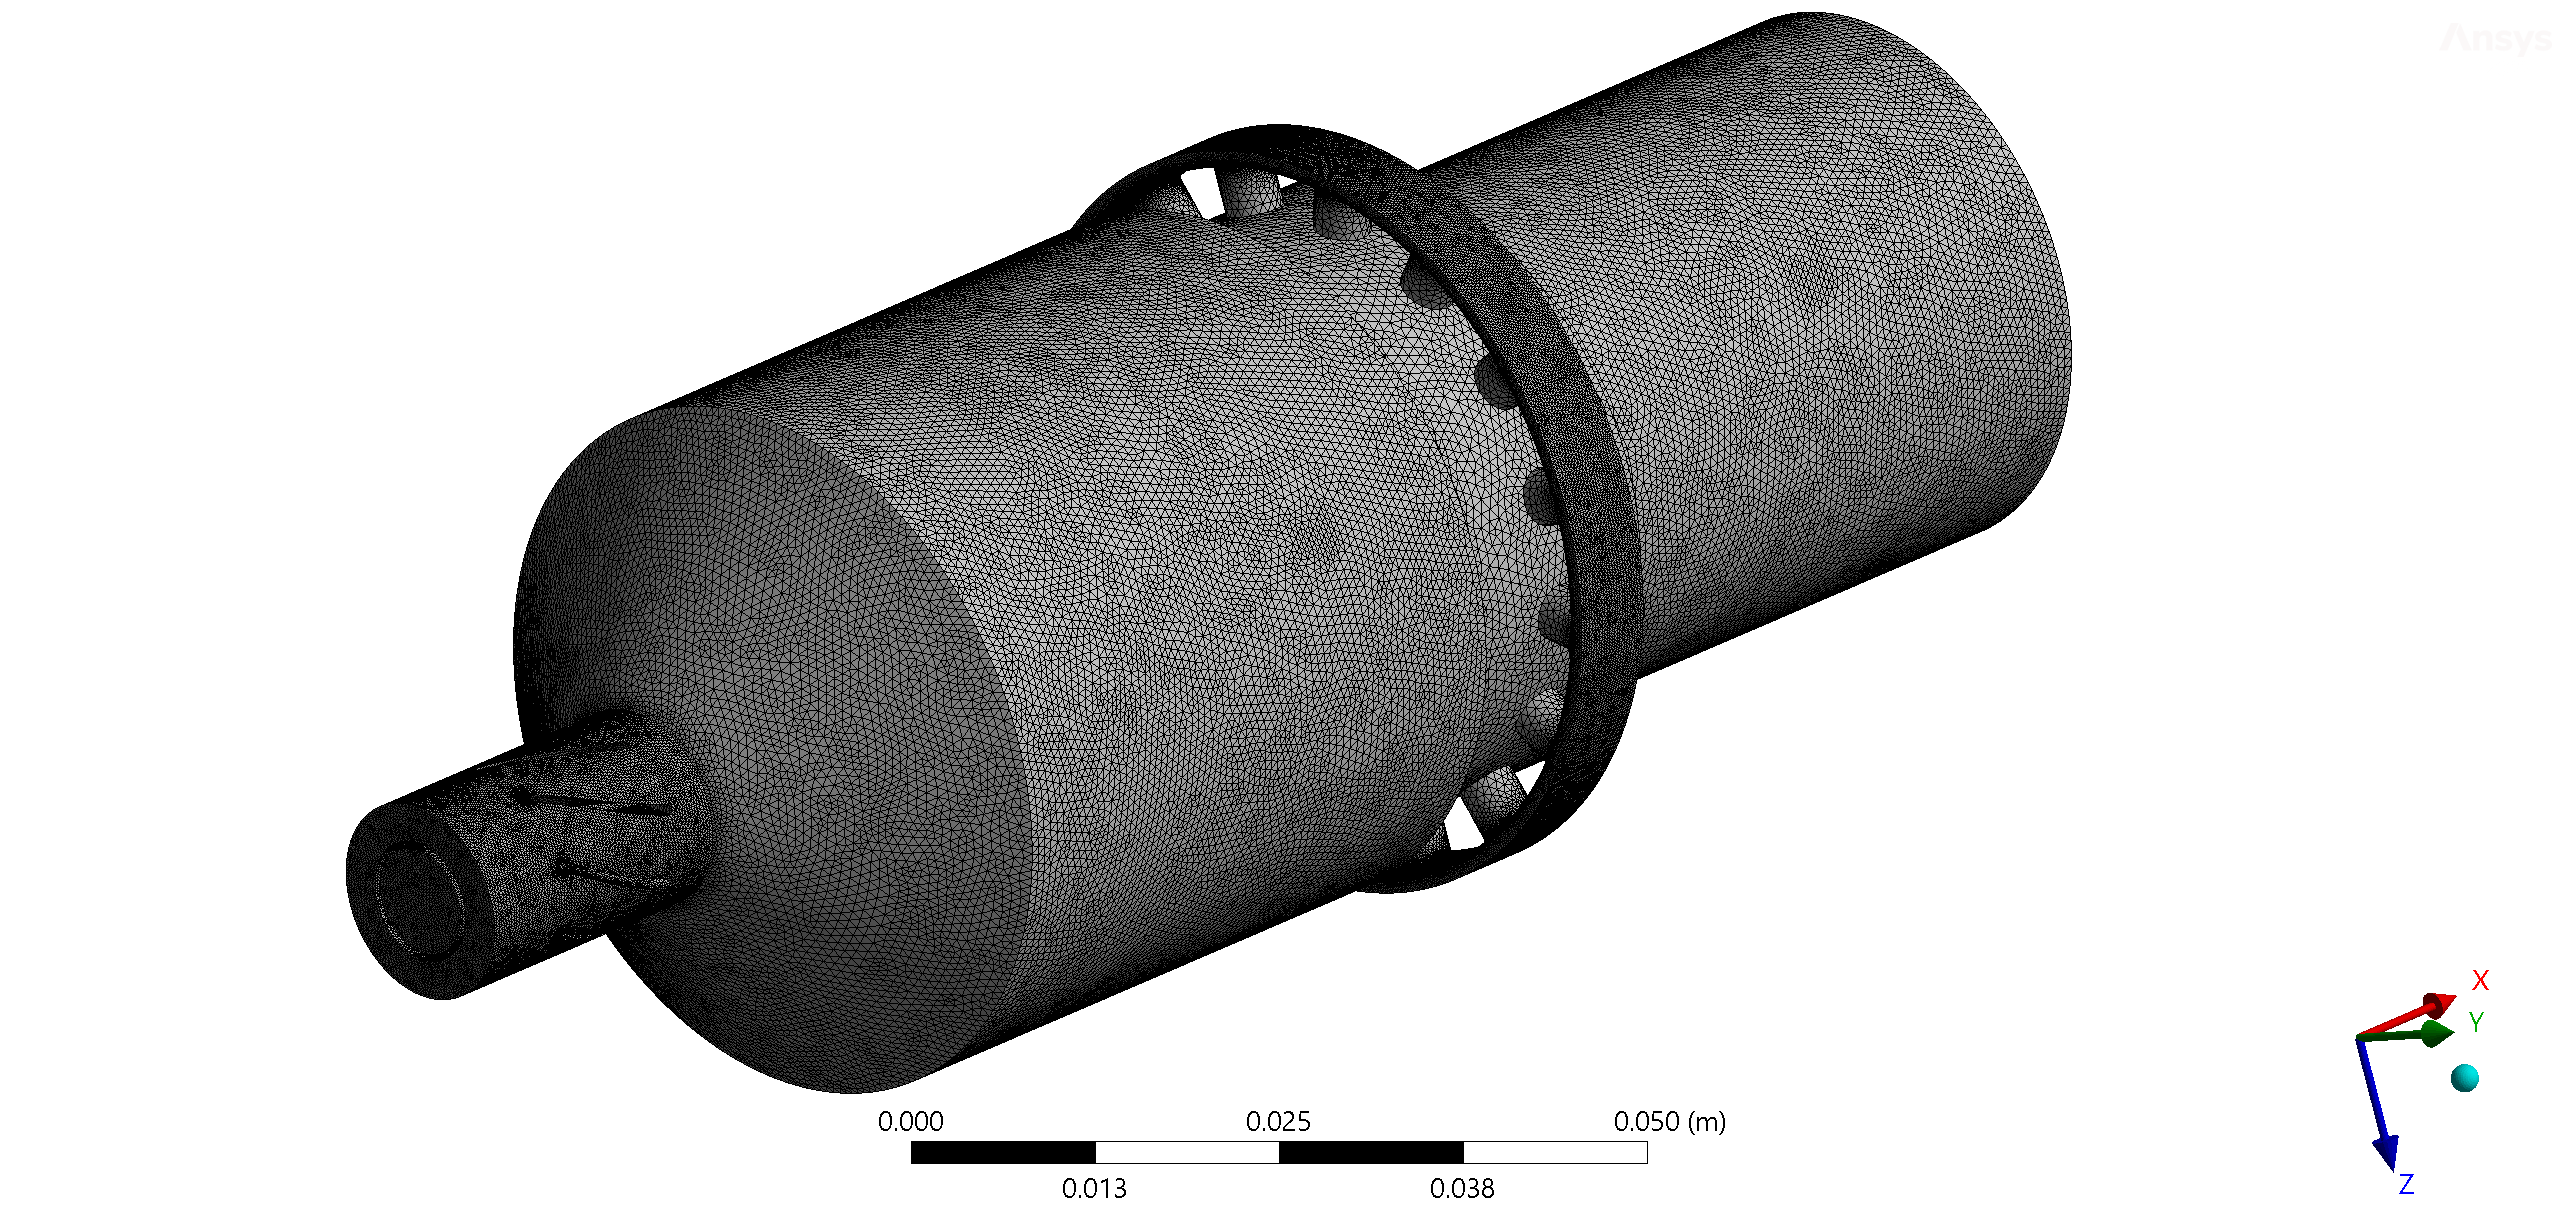
\includegraphics[width=\textwidth]{figs/mesh.png}
    \caption[]%
    {{\small Overall mesh.}}    
\end{subfigure}
\hfill
\begin{subfigure}[b]{0.49\textwidth}   
    \centering 
    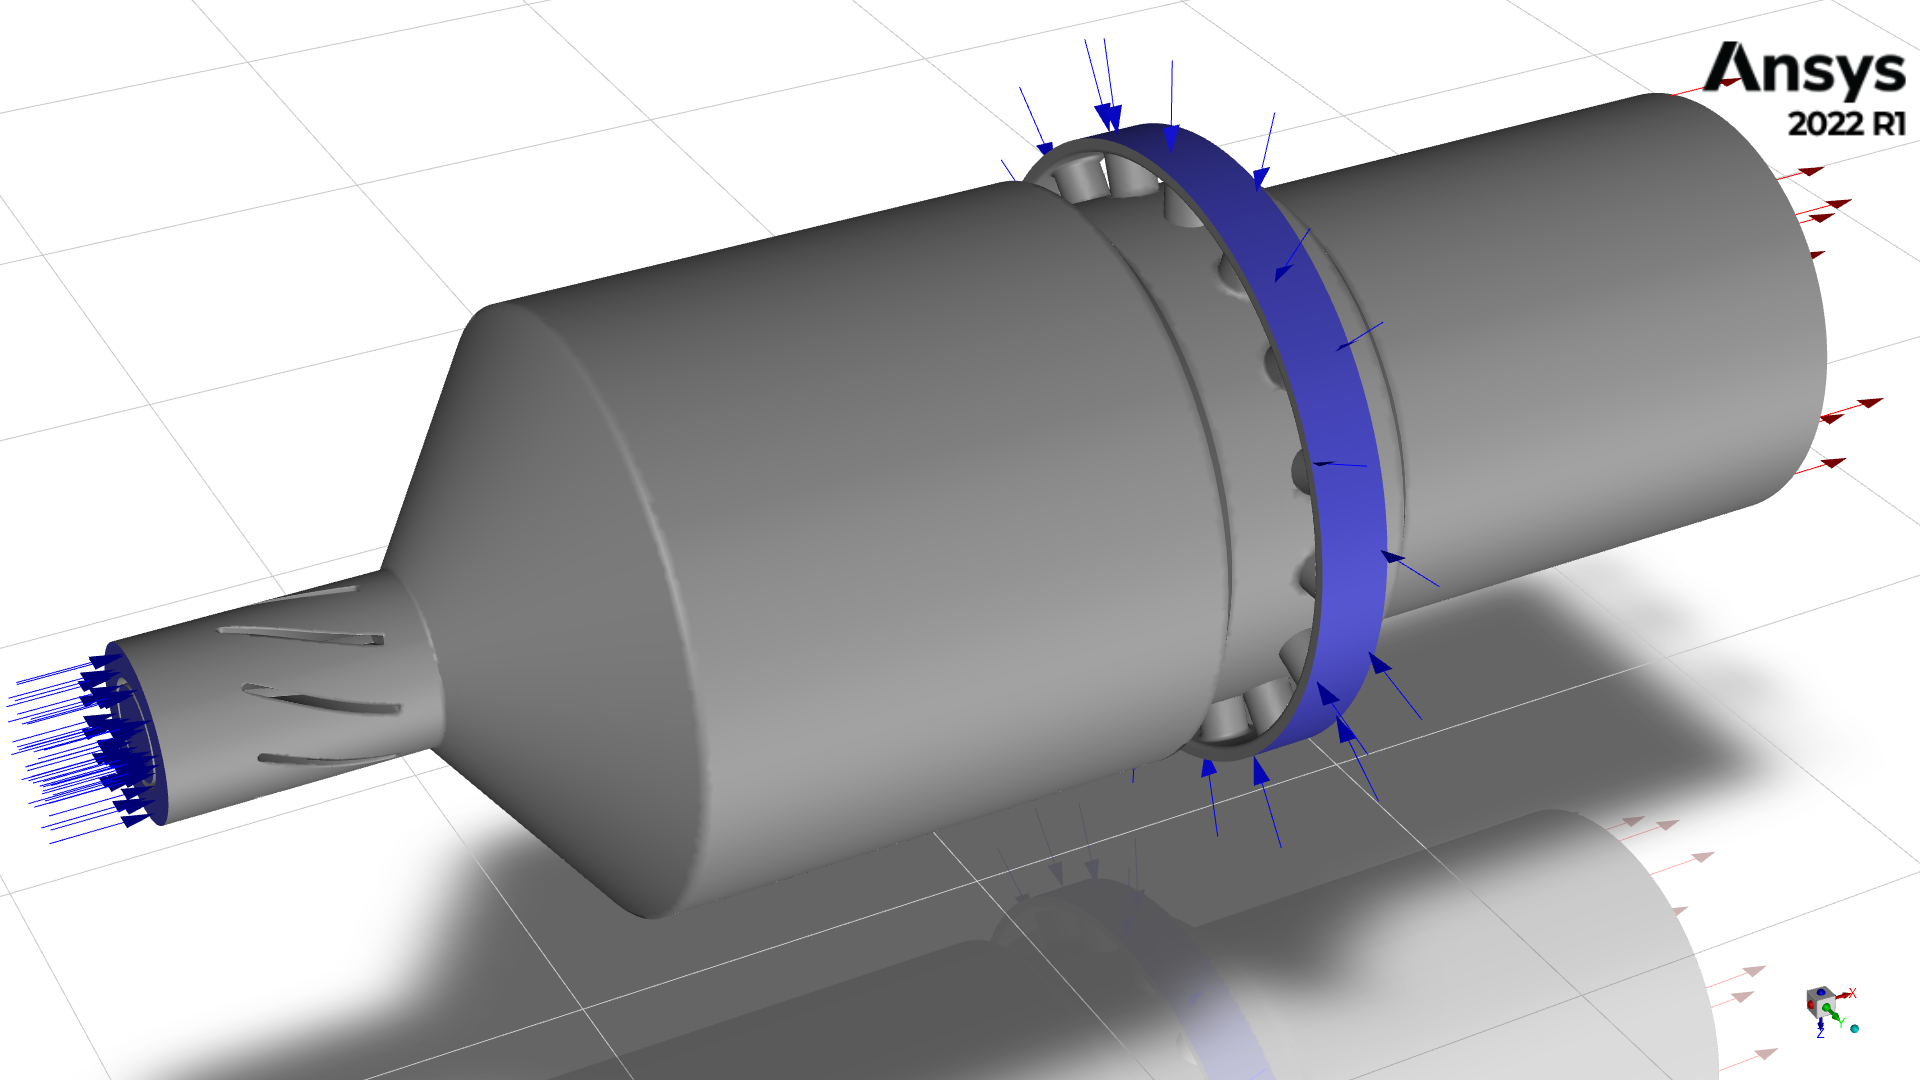
\includegraphics[width=\textwidth]{figs/bound_cond.png}
    \caption[]%
    {{\small Boundary conditions.}}    
\end{subfigure}
\caption{Numerical mesh and setup.} 
\label{fig:numerical_setup}
\end{figure}


\subsubsection{Setup}

To simulate reacting flow, the energy model is turned on. Additionally, the combustion model is set to non-premixed combustion. The settings used are shown in \autoref{fig:setups_lol}. 


\begin{figure}[H]
\centering
\begin{subfigure}[b]{0.49\textwidth}   
    \centering 
    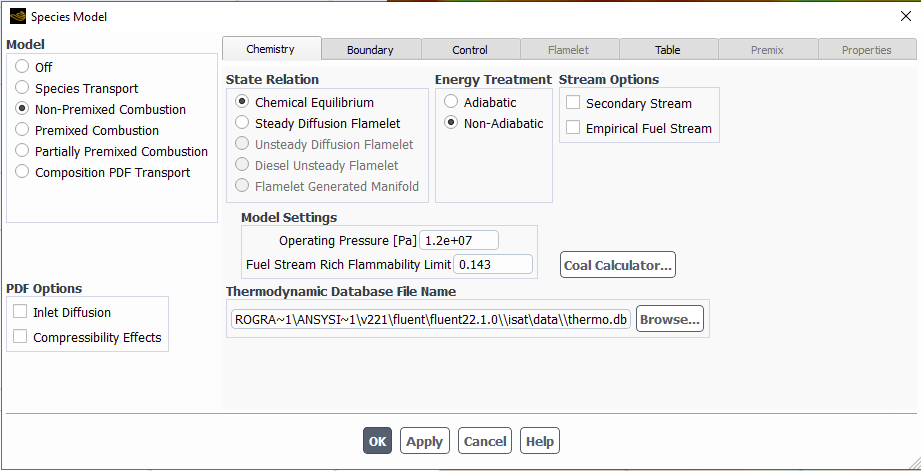
\includegraphics[width=\textwidth]{figs/setup_1.png}
    \caption[]%
    {{\small Setup for chemistry.}}    
\end{subfigure}
\hfill
\begin{subfigure}[b]{0.49\textwidth}   
    \centering 
    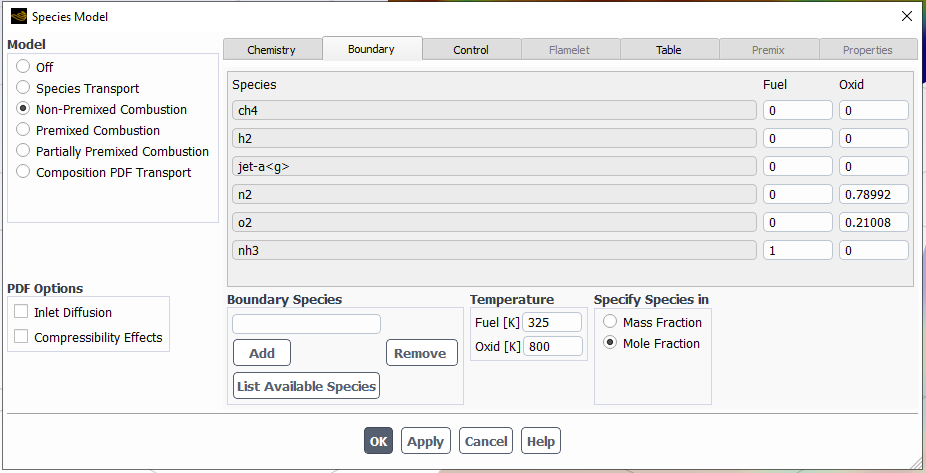
\includegraphics[width=\textwidth]{figs/setup_2.png}
    \caption[]%
    {{\small Setup for boundary.}}    
\end{subfigure}
\caption{Non-Premixed combustion setup.} 
\label{fig:setups_lol}
\end{figure}

